\documentclass{article} % For LaTeX2e
\usepackage{iclr2018_conference,times}
\usepackage{url}
\usepackage{amsthm}
\usepackage{algorithm}
\usepackage{algorithmic}
\usepackage{times}
\usepackage{graphicx}
\usepackage{color}
\usepackage{amsmath}
\usepackage{amsfonts}
\usepackage{url}
\usepackage{textcomp}
\usepackage{amsthm}
\usepackage{float}

\frenchspacing

\def\presentationmode{1}

\def\beginFrame#1{\if\presentationmode1 \begin{frame}{#1} \else \fi}
\def\endFrame{\if\presentationmode1 \end{frame} \else \fi}

\newcommand{\mat}[1]{\mathrm{\mathbf{#1}}}
\newcommand{\vect}[1]{\mathrm{\mathbf{#1}}}
\newcommand{\fros}[1]{\left\| #1 \right\|_\mathrm{F}^2}
\newcommand{\Expect}[2]{\mathbb{E}_{#1}\left[ #2 \right]}
\newcommand{\KL}[2]{ \mathrm{KL}\left( #1 \| #2 \right) }
\newcommand{\Real}{\mathbb{R}}
\newcommand{\T}{\mathrm{T}}
\newcommand{\tr}{\mathrm{tr}}
\newcommand{\sigmoid}{\sigma}
\newcommand{\Simga}{\Sigma}
\newcommand{\attention}{\vect{g}}
\def\attentionwithouti{g_2, \dots, g_k}
%\def\attentionwithouti{\boldsymbol{\gamma}_{i}}
\newcommand{\attraction}{\vect{h}}

\def\x{\vect{x}}
\def\y{\vect{y}}
\def\h{\vect{h}}
\def\g{\vect{g}}
\def\s{\vect{s}}
\def\c{\vect{c}}
\def\A{\mathcal{A}}
\def\S{\mathcal{S}}
\def\R{\mathcal{R}}
\def\Trans{\mathcal{T}}
\def\E{\mathcal{E}}
\def\deriv#1#2{ \frac{\partial #2}{ \partial #1 } }
\def\derivN#1#2#3{ \frac{\partial^{#1} #3}{ \partial #2^{#1} } }
\def\grad#1#2{ \deriv{#1}{#2} }
\def\gradN#1#2#3{ \derivN{#1}{#2}{#3} }
\def\Grad#1#2{ \nabla_{#1} {#2} }
\def\obs{\vect{o}}
\def\u{{\boldsymbol{b}}}
\def\w{{\boldsymbol{\alpha}}}
\def\vmu{{\boldsymbol{\mu}}}
\def\v{\vect{v}}
\def\g{\attention}
\def\h{\attraction}
\def\G{\mat{G}}
\def\op{}
%\def\Qg{Q^{\mathrm{g}}}
%\def\ug{\vect{u}^{\mathrm{g}}}
\def\Qg{Q}
\def\ug{\u}
\def\params{{\boldsymbol{\theta}}}
\def\Params{{\boldsymbol{\Theta}}}
\def\opt#1{{\hat{#1}}}
\def\argmax{\mathrm{argmax}}

%\def\costof#1{C(#1)}
\def\costof#1{\mathrm{C}[{#1}]}
\def\budget{B}
\def\cost{c}
\def\vcost{\vect{\cost}}
\def\costat#1{\cost_{#1}}
\def\costi{c_i}
\def\unit{\vect{e}}
\def\units{k}
\def\state{\s}
\def\action{a}
\def\rewards{y}

\def\sumk#1{\sum_{#1=1}^k}
\def\Si{\sumk{i}}
\def\Sj{\sumk{j}}

\def\vcatout{\tilde{\vect{h}}}
\def\catout{\tilde{h}_i}
\def\catoutj{\tilde{h}_j}
\def\changeof#1{\Delta #1}

\def\vcatin{\vect{h}}
\def\catin{h_{i}}
\def\catinj{h_{j}}

\def\vcatbias{\vect{h}_i}
\def\catbias{\mu_i}
\def\catbiasj{\mu_j}

\def\qbias{q_i}
\def\vqbias{\mathbf{q}}
\def\qin{Q}

\def\ebias{e_{-i}}
\def\ein{e}
\def\changeofebias{{\changeof\qbias} \left[ \changeof\qbias + 2 \TDerror{\qin} \right]}
%\def\changeofebias{{\changeof\qbias}\left( \changeof\qbias + 2 \delta_t \right)}

\def\regret{\rho_{-i}}
%\def\TDerror#1{E_{\mathrm{TD}}\left({#1}\right)}
\def\TDerror#1{\delta}


\def\prA{p(\rewards|\state, \action, \params, \g)}
\def\LLAttention{\log \prA}

\def\Square#1{\left[ #1 \right]^2}

\def\ReplayMemory{\mathcal{D}}
\def\play{\s_t, a_t, r_t, \s_{t+1}}
\def\Play{(\play)}
\def\pl{\mathsf{d}_t}
\def\Replays#1{\Expect{ \pl \sim \ReplayMemory}{#1}}

\def\bUpdate#1{p(o_{t+1}|s_${#1},a_t) \sum_i p(s_{#1}|s_i, a_t) b_{t}^i}
\def\beliefState#1{ \vect{b}_{#1} }

\def\const{\mathrm{const.}}
\def\test{_\mathrm{test}}
\def\train{_\mathrm{train}}
\def\bs{\boldsymbol}
\def\etal#1{{et al.} (\citeyear{#1})}
\def\Etal{{et al.}}
\def\Long{1}
\def\eg{e.g., }

\def\eAt#1{e_{#1}}
\def\eBase{\eAt{\one}}
\def\one{\mathbf{1}}
\def\zero{\mathbf{0}}
\def\unit#1{\vect{u}_{#1}}
\def\eChange#1{ \Delta e_{#1} }

\def\ask{q}


% probability
\def\prob#1{p\left(#1\right)}
\def\prob#1#2{p\left(#1 \mid #2 \right)}

\def\deprecated{\alert{[Deprecated]}}
\def\softmax{\mathrm{softmax}}


\newcommand{\penalvec}[3]{ \frac{1}{2 \sigma_#1^2} \sum_{#2=1}^{#3} \vect{#1}_{#2}^\T  \vect{#1}_{#2} }

\newcommand{\CON}{\color{red}}
%\newcommand{\CON}{\color{black}}
\newcommand{\COFF}{\color{black}}

%\newcommand{\CON}{\color{red} -------- My modification starts from here. ------- \color{black}}
%\newcommand{\CON}{\color{black}}
%\newcommand{\COFF}{\color{red} -------- My modification ends here. ------- \color{black} }


\newtheorem{thm}{Theorem}[section]
\newtheorem{coro}{Corollary}[section]
\newtheorem{prf}{Proof}
\newtheorem{defn}{Definition}



\title{Neuron as an Agent}

%\author{Shohei Ohsawa, Kei Akuzawa, Yusuke Iwasawa \& Yutaka Matsuo \\
%The University of Tokyo\\
%7 Chome-3-1 Hongo, Bunkyo, Tokyo \\
%\texttt{ohsawa@weblab.t.u-tokyo.ac.jp} \\
%}
\author{Anonymous}

\newcommand{\fix}{\marginpar{FIX}}
\newcommand{\new}{\marginpar{NEW}}

\begin{document}

\maketitle

\begin{abstract}
We propose {\em Neuron as an Agent} (NaaA) as a novel framework for deep multi-agent reinforcement learning (MARL),
which incorporates all neural network units as agents and optimizes the reward distribution. % as a MARL problem.
NaaA deals with reward distribution among the agents by combining MARL with economics.
%First, showing optimization of NaaA, this report describes the negative result that the performance decreases if we naively consider the units as agents.
%To resolve that difficulty, we introduce a mechanism from game theory.
As a theoretical result, we demonstrate that the agent obeys the system to maximize its {\em counterfactual return} as the Nash equilibrium of the mechanism.
Subsequently, we show that learning counterfactual returns leads the model to learning optimal topology among units, and improves performance of a single-agent RL task.
We propose {\em adaptive dropconnect}, a natural extension of dropconnect.
Finally, we confirm that optimization with the framework of NaaA leads to better performance of RL, with numerical experiments.
Specifically, we use a single-agent environment from Open AI gym, and a multi-agent environment from ViZDoom.
\end{abstract}

\section{Introduction}
Recent successful results of deep reinforcement learning (DRL) in TV games \citep{mnih2015human} and board games \citep{silver2016mastering} are supported by capability of a deep neural network to obtain good state representation by abstracting high-dimensional input. %such as a screen and a board face.
Unlike these artificial environments, applying DRL to industry such as mobility, finance and agriculture requires way to observe state representation in a partially observed environment.
In addition to predicting unobserved state which reports reasonable performance in partially observed environment such as a first-person shooting game \citep{dosovitskiy2016learning},
multi-agent reinforcement learning (MARL) is an emerging topic to observe wider range of state with communication.
Several researchers proposed methods to learn appropriate communication as a cooperative setting \citep{sukhbaatar2016learning}.
 %is a method for cooperative MARL to learn multi-agent communication among agents with common objective.
%the real environment cannot be completely observed by single agent.

What is unsolved by these communication methods in MARL is reward distribution for configuration in which agents are not cooperative but selfish.
Considering an environment such as Web, these agents will be developed by different people and companies with different objective.
Hence, they are not incentivesed to develop an agent without an appropriate reward distribution.
As the recent work \citep{sukhbaatar2016learning} considers whole multi-agent system with communication as a neural network,
this discussion for incentive is reduced to consider a unit as an agent ultimately.
% equivalent to asking the following question.
%Eventually, the problem is dealt with by answering the following question.
%MARL allows each agents made of a single unit.
Therefore, we address the following question.
%CommNet considers an agent as an neuron, and train the communication between the agents with back propagation.

\begin{center}
{\em Will reinforcement learning work even if we consider each unit as a selfish agent?}
\end{center}

The contribution of this paper is that we propose {\em Neuron as an Agent} (NaaA) as a novel framework for RL, and its optimization method.
NaaA incorporates all neural network units as agents and optimizes the reward distribution as a multi-agent RL problem.
In the reward design of NaaA, a unit distributes its received reward as cost to other input units in order to observe their activation.
Consequently, the actual reward is profit, defined as the difference between inflow (received reward) and outflow (paid cost).
In the setting, the economic metaphor can be introduced: profit is the balance of revenue and cost. 
%There are several point to discuss for the reward distribution:
%"How much the reward is appropriate per agent" and "How to obligate agents to distribute reward."
%The one is known as credit assignment problem in multi-agent reinforcement learning (MARL), and
%the another one ks also known as a treatment of social dilemma.
%Recently, emerging technology of blockchain enabled us to distribute reward to agents with cryptocurrency such as bitcoin and ethereum.
The source of reward is from reward which the actuator obtain by obtaining good state representation from the environment.

%====================================================================================
% �����͂��̂܂܂ł悢
This paper is organized as presented below.
First, showing the optimization of NaaA, this report describes the negative result that the return (cumulative discounted reward) decreases if we naively consider units as agents.
As a solution to this difficulty, we introduce a mechanism of auction which applies game theory.
As a theoretical result, we demonstrate that the agents maximize their {\em counterfactual return} in Nash equilibrium.
The counterfactual return is that by which we extend counterfactual reward, the criterion proposed for multi-agent reward distribution problem \citep{agogino2006quicr}, along a long time axis.

Subsequently, we present that maximizing counterfactual return leads the model to learning optimal topology between the units with respect to supervised learning as well as RL.
In addition, we propose {\em adaptive dropconnect}, a natural extension of dropconnect \citep{wan2013regularization}.
Adaptive dropconnect combines dropconnect, which randomly masks the topology, with an adaptive algorithm, which prunes connections with less counterfactual return with higher probability.
It uses $\varepsilon$-greedy as a policy, and is equivalent to dropconnect in the case of $\varepsilon = 1$. It is equivalent to counterfactual return maximization, which constructs the topology deterministically in the case of $\varepsilon = 0$.

Finally, we confirm that optimization with the framework of NaaA leads to better performance of RL, with numerical experiments.
Specifically, we use a single-agent environment from Open AI gym, and a multi-agent environment from ViZDoom.
%====================================================================================

Although considering all the units as agents might be simplistic at first glance, it has a wider applicable area.
From the perspective of optimization for a single neural network, it can be applied to pruning by optimizing the topology.
Furthermore, introducing the concept of reward distribution divides the single neural network to numerous autonomous parts.
It enables us not only to address sensor placing problem in IoT for partially observed Markov decision process (POMDP): arbitrary incentivized participants can join the framework.

%We focus on DRL in the multi-agent setting.
%Deep Deterministic Policy Gradient (DDPG) \citep{lillicrap2015continuous} realizes the multiple-join control considering conditions such as friction and gravity factors in a physical space.
%The applicability of DRL is becoming wider year by year. Reasonable performance is reported for 3D games such as Doom \citep{dosovitskiy2016learning}.
%Applying DRL to industry such as mobility, finance and agriculture as people expected, requires curious way to observe environment.

%The problem can be solved by two approaches.
%The one is predicting transition of unobserved state by neural network,
%which achieved by an agent with a recurrent model such as a recurrent neural network to explore
%the environment actively to obtain information.
%The another one is to prepare multi-agent environment to observe environment indirectly by communication.

%\section{Background}
First, we consider a POMDP environment in which a single agent acts.
The POMDP environment is a seven-tuple $(\S, \A, \Trans, \R, \Observations, \ObProb, \gamma)$,
where $\S$ represents a set of states, $\A$ stands for a set of actions, $\Trans$ denotes a transitive probability, 
$\R: \S \times \A \rightarrow \Real $ is a function from the state and the action of an agent to the real value.
$\Observations$ represents a possible set of observations, $\ObProb$ denotes a set of observation probability, and
$\gamma$ is the discount rate.
An agent partially predicts state $h \in \S$ through an observation $s \in \Observations$.

Generally, $s$ has higher dimensions than $h$, and is complex.
For example, although Atari 2600 has a read only memory (RAM) as the true state, which contains 128 bytes,
the generated image from that $s$ has more than 10,000 dimensions.
Therefore, DQN and DRQN abstract $s$, and create original state representation to predict good action efficiently.
(Although the original paper of DQN assumes MDP, the paper of DRQN pointed out that the environment is POMDP).
Although DQN does not address the state transition directly because it is model-free method, 
some interpretations hold that the hidden state representation is learned in the previous layer of the output layer \citep{zahavy2016graying}
Using the method below, we assume that the agent chooses an action through a neural network.
The POSG environment is a natural extension of POMDP to multi-agent environment defined by a tuple $(\S, \A^i, \Trans, \R^i, \Observations^i, \ObProb^i, \gamma^i)_{i \in \mathcal{I}}$,
where $\mathcal{I}$ is a finite set of agents indexed 1, \dots, $N$.
Each agent has a policy $\pi_i: \Observations^i \rightarrow \A^i$. 
They maximize their return by interacting with the environment.

%The POSG environment is a multi-agent environment defined by a tuple $(\S, \A^i, \Trans, \R^i, \Observations^i, \ObProb^i, \gamma^i)_{i \in \mathcal{I}}$,
%where $\mathcal{I}$ is a finite set of agents indexed 1, \dots, $N$, 
%$\S$ represents a set of states, 
%$\A^i$ stands for a set of actions, 
%$\Trans$ denotes a transitive probability, and 
%$\R^i: \S \times \A^1 \times \cdots \times \A^N \rightarrow \Real $ is a function from the state and the action of all agents to the real value.
%$\Observations^i$ represents a possible set of observations. $\ObProb^i$ denotes a set of observation probability.
%$\gamma^i$ is the discount rate.
%Each agent has a policy $\pi_i: \Observations^i \rightarrow \A^i$. They maximize their return by interacting with the environment.
%A difference from POMDP is that there are $N$-agents.

We employ several concepts from game theory.
Although RL and game theory are typically investigated in parallel, several concepts in game theory can be written in the domain of RL.
The (Bayesian) Nash equilibrium $\hat{\pi}_{i}$ is a policy by which all agents maximize their expected reward. That is,
\begin{flalign}
\hat{\pi}(s_{it}) = \argmax_{a_i \in \A^i} \Expect{ \vect{a}_{-i} \in A^{-i}, h \sim \ObProb^i }{ \R^i(h, \vect{a}) | s_{it}} \, \forall i \in \mathcal{I},
\end{flalign}
where $\mathcal{A}^{-i}$ is a set of actions except for $i$. 
Intuitively, the equation took an expected value of reward to integrate out other agents' unobserved actions.
Because the Nash equilibrium is sufficient to state only the best action in the most cases, we use the notation with action $\hat{\vect{a}}$ in the following.


\section{Neuron as an Agent}
%TODO: Show the figure.
% ���̏͂ł�������
% �E�j���[�������G�[�W�F���g�Ƃ݂Ȃ�
% �E�����‚��̑O����Ă���
% �ENaaA �� social welfare function ���ő剻���邱�Ƃ��A�O������̃����[�h�ő剻�Ɉ�v����B

\subsection{Problem Definition}
Suppose there are $N$ agents interacting to an environment. 
%This paper addresses reward distribution problem at multi-agent communication among the agents.
Some agents get reward from the environment, and distribute it to other agents as incentive to give precise information.
The reward is limited so that if an agent distribute $\rho$ reward, the agents' reward subtracted by $\rho$ such as currency.
For the reason, other agents for an agent itself can be interpreted as another environment which 
give a reward $-\rho$ instead of an observation $x$.
We name the another environment as {\em internal environment} and name the original environment as an {\em external environment}.

Our goal is to maximize the discounted cumulative reward which the system will obtain from the external environment.
 %total discounted cumulative reward from the external environment which all the $N$ agents will obtain.
\begin{equation}
%G^\mathrm{ex} = \sum_{i=1}^n \left[ \sum_{k=0}^T \gamma^k R_{i,k+t}^\mathrm{ex} \right],
G = \sum_{i=1}^n \left[ \sum_{t=0}^T \gamma^k R_{it}^\mathrm{ex} \right],
\end{equation}
where $R_{it}^\mathrm{ex}$ is an external reward which $i$-th agent obtains at $t$, and $\gamma \in [0, 1]$ is the discount rate and $T$ is the terminal time.

Similarly to CommNet \citep{sukhbaatar2016learning}, we assume that the communication protocol between the agent is a continuous quantity such as a vector, and the content can be trained by backpropagation.
Hence, we can interpret the multi-agent communication as a huge neural network.
Therefore, we can interpret a unit as an agent without loss of generality.
This framework can single-agent reinforcement learning as well as multi-agent reinforcement learning.

\subsection{The Framework}
A typical artificial neural network is a directed graph $\neuralnet = (\units, \edges)$ among the units.
$\units = \{\unitAt{1}, \dots, \unitAt{N}\}$ is a set of the units. $\edges \subset \units^2$ is a set of edges representing connections between two units.
If $(\unit, \unitAt{j}) \in \edges$, then connection $\unit \rightarrow \unitAt{j}$ holds, indicating that $\unitAt{j}$ observes activation of $\unit$.
We denote activation of the unit $\unit$ at time $t$ as $x_{it} \in \Real$.
Additionally, we designate a set of units which unit $i$ connects to as $\followers = \{j | (\unit, \unitAt{j}) \in \edges \}$ and a set of units which unit $i$ is connected from as $\followees = \{j | (\unitAt{j}, \unit) \in \edges \}$.
We denote $\friends = \followees \cup \followers$.

NaaA interprets $\unit$ as an agent.
Therefore, $\neuralnet$ is a multi-agent system.
An environment for $\unit$ comprises an environment that the multi-agent system itself touches and a 
set of the unit to which $\unit$ directly connects: $\{v_i \in \units | i \in \friends\}$.
We distinguish both environments by naming the former as an external environment, and by naming the latter as an internal environment.
$\unit$ will receive rewards from both environments.
We add the following assumption for characteristics of the $\unit$.
\begin{enumerate}
\renewcommand{\labelenumi}{N\arabic{enumi}:}
\item (Selfishness) 
	The utility which an $\unit$ wants to maximize is its own return (cumulative discounted reward):
	$G_{it} = \sum_{k=0}^T \gamma^k \rewardAt{i,t+k}$.
\item (Conservation) 	% Energy Conservation
	The summation of internal reward over $\units$ equals to 0.
	Hence, the summation of a reward by which $\units$ will receive both an internal and external environment $\reward$ are equivalent to reward $R_t^{\mathrm{ex}}$, which the entire multi-agent system receives from the external environment.
\item (Trade) 
	The $\unit$ receives internal reward $\rho_{jit}$ from $\unitAt{j} \in \units$ in exchange of activation signal $x_i$
	before transferring the signal to the unit. At the same time, $\rho_{jit}$ is subtracted from the reward of $v_j$.
\item (NOOP) 
	$\unit$ has NOOP (no operation), for which the return is $\delta > 0$ as an action.
	With NOOP, the unit inputs nothing and outputs nothing.
\end{enumerate}
In terms of neuroscience,
N1 states that the unit acts as a cell.
N2 and N3 state the distribution of NTF. N4 corresponds to apoptosis.
NOOP is selected when the expected returns of the other actions are non-positive.
In the following, we construct the framework of NaaA from the assumptions.

The social welfare function (total utility of the agents) $G^\mathrm{all}$ is equivalent to the objective function $G$. That is,
\begin{equation}
	G^\mathrm{all} = \sum_{i=1}^n G_{it} = \sum_{i=1}^n \left[ \sum_{k=0}^T \gamma^k R_{it} \right] 
		= \sum_{k=0}^T \left[ \gamma^k \sum_{i=1}^n R_{it} \right].
\end{equation}
From N2, $\sum_{i=1}^n R_{it} = \sum_{i=1}^n R_{it}^{\mathrm{ex}}$ holds. Hence, $G^\mathrm{all} = G$ holds.
%\begin{equation}
%	G^\mathrm{all} = \sum_{k=0}^T \left[ \gamma^k \sum_{i=1}^n R_{it}^{\mathrm{ex}} \right] = G.
%\end{equation}

%================================================================
\subsection{Cumulative Discounted Profit Maximization Framework}
%================================================================
We denote the external reward by which unit $\unit$ receives at time step $t$ as $R_{it}^\mathrm{ex}$, where $\sum_{i=1}^n R_{it}^\mathrm{ex} = R_t^{\mathrm{ex}}$ holds.
From N3, reward $R_{it}$, which $\unit$ receives at $t$ can be written as the following.
\begin{flalign}
	R_{it} = 
	  R_{it}^\mathrm{ex} + \sum_{j \in N^\mathrm{out}_i} \rho_{jit} 
	- \sum_{j \in N^\mathrm{in}_i} \rho_{ijt}.
\end{flalign}
The equation is divided into positive terms and a negative term, we name the former as revenue, and the latter as cost, and denote them respectively as $r_{it} = R_{it}^\mathrm{ex} + \sum_{j \in N^\mathrm{out}_i} \rho_{jit}, \, c_{it} = \sum_{j \in N^\mathrm{in}_i} \rho_{ijt}$.
We name $R_{it}$ as profit.


$\unit$ maximizes the cumulative discounted profit $G_{it}$ represented as
\begin{flalign}
	G_{it}	= \sum_{k=0}^T \gamma^k R_{i, t+k} 
			= \sum_{k=0}^T \gamma^k (r_{i,t+k} - c_{i,t+k})
			&= r_t - c_t + \gamma G_{i,t+1}.
\end{flalign}
$G_{it}$ is unobserved unless the time is reached at the end of the episodes.
Because prediction based on the current value is needed to select the optimal actions, 
we approximate $G_{it}$ with value function $V_i^{\pi_i} (s_{it}) = \Expect{\pi_i}{ G_{it} \mid s_{it}}$ where $s_{it} \in \Observations$.
In this case, the following equation holds.
\begin{flalign} 
		V_i^{\pi_i} (s_{it}) = r_{it} - c_{it} + \gamma V_i^{\pi_i} (s_{i, t+1}),	\label{eq:V}
\end{flalign}
Therefore, we need only consider maximization of revenue, the value function, and cost minimization.
$R_{it} > 0$, i.e., $r_{it} > c_{it}$ indicates that the unit gives the additional value to the obtained data.
The unit acts NOOP because $V_i^{\pi_i} (s_{it}) \leq 0 < \delta$ if $R_{it} \leq 0$ for all $t$ because of N4.

%TODO: verify equation of V



%The design of NaaA is inspired by neuroscience.
%A neuron in a neurocircuit consumes adenosine triphosphate (ATP) supplied from connected astrocytes.
%The astrocyte is a glia cell, which forms the structure of a brain. It supplies fuel from the vessel.
%Because the amount of ATP is constrained, the discarded neuron will become extinct with execution of apoptosis.
%Also, because apoptosis of a neuron is restrained by neurotrophins (NTFs) such as nerve growth factor (NGF) and brain-derived neurotrophic factor (BDNF),
%neurons which can obtain much NTF will live.
%The perspective of interpreting a neuron as an independent living object is known as neural Darwinism \citep{edelman1987neural}.

\section{Auction Theory}
%To maximize the cumulative discounted profit in a framework of NaaA,
%it is important to balance the two contradicting criteria: revenue $r_{it}$ and cost $c_{it}$.

%TODO:
% ・語られていない前提: R_ex は出力ユニットにのみ配分される
% ・語られていない前提: どんなゲームを行うのか(必要なアクションは何か)

%TODO: Negative result. State what is the problem.
%\begin{thm}\label{thm:optimal-bidding-simple}
%$\pi_i$ is the Nash equilibrium if and only if $\rho_{ijt} = 0$ regardless $\neuralnet$
%\end{thm}
%(TODO: Bad writing.)
We introduce mechanism design because, unlike several existing studies \citep{sukhbaatar2016learning}, NaaA assumes that all agents are not cooperative but selfish.
If we naively optimize the optimization problem of NaaA, then we obtain the trivial solution that the internal rewards will converge to 0, and that all the units except of the output units become NOOP.
This phenomena occurs regardless the network topology $\neuralnet$ as any nodes have no incentive to send payment $\rho_{ijt}$ to other units.
Therefore, the multi-agent system should select the action with no information. It is equivalent to taking an action randomly.
For that reason, the external reward $R_t^{\mathrm ex}$ shrinks markedly.

\subsection{Envy-free Auction}
To maximize the overall reward, our objective function, we borrow the idea from the digital goods auction.
The auction theory belongs to mechanism design. It is intended to unveil the true price of goods.
Digital goods auction is one mechanism from auction theory.
It is target to copyable goods without cost, such as digital books and music.

Although several variations of digital goods auctions exist,
we use an envy-free auction \citep{guruswami2005profit} because it requires a simple assumption: the same goods have one price simultaneously.
In NaaA, it can be represented as the following assumption:
\begin{enumerate}
\renewcommand{\labelenumi}{N\arabic{enumi}:}
\setcounter{enumi}{4}
\item (Law of one price)
	If $\rho_{j_1,i,t}, \rho_{j_2,i,t} > 0$, then $\rho_{j_1,i,t} = \rho_{j_2,i,t}$.
\end{enumerate}
The assumption above indicates that $\rho_{jit}$ takes either 0 or a positive value depending on $i$ at a same timing $t$.
Therefore, we name the positive side $\unit$'s {\em price}, and denote as $q_{it}$.

%TODO: Describe for allocation

We present the envy-free auction process at the left of Figure \ref{fig:double}.
It shows the negotiation process between one unit in sending activation and a group of units that buy the activation.
The negotiation performed per time step in RL.
We name the unit in sending activation as a seller, and units in buying activation as buyers.
First, the buyer bids the unit in bidding price $b_{jit}$ (\textbf{1}).
Next, the seller decides the optimal price $\opt{q}_{it}$, and performs allocation (\textbf{2}).
Payment occurs if $b_{ijt}$ exceeds $q_{jt}$.
In this case, $\rho_{jit} = H(b_{jit} - q_{it}) q_{it}$ holds where $H(\cdot)$ is a step function.
Besides, we define $g_{jit} = H(b_{jit} - q_{it})$ and name it {\em allocation}.
After allocation, the buyers perform payment as $\rho_{jit} = g_{jit} \opt{q}_{it}$ (\textbf{3}).
Eventually, seller earns 
The seller only sends activation $x_i$ to the allocated buyers (\textbf{4}).
A buyer which cannot receive the activation approximates $x_i$ with $\Expect{\pi}{x_i}$.

In the following, we discuss revenue, cost, and value functions based on Eq:(\ref{eq:V}).



%========================================
% 収益
%========================================

\textbf{Revenue}:
The revenue of a unit is given as
\begin{flalign}
	r_{it}  = \sum_{j \in N^\mathrm{out}_i} g_{jit} q_{it} + R^\mathrm{ex}_i 
		= q_i d_{it} + R^\mathrm{ex}_i,
\end{flalign}
where $d_{it} = \sum_{j \in N^\mathrm{out}_i} g_{jit}$ is a count of units for which the bidding price for $q_{it}$ is greater than or equal to $q_{it}$, designated as demand.
$q_{it}$ maximizing the equation is designated as the optimal price. It is denoted as $ \opt{q}_{it} $.
Because $R^\mathrm{ex}_i$ is independent of $q_t$, the optimal price $\opt{q}_{it}$ is given as
\begin{flalign}
	\opt{q}_{it}  = \argmax_{q \in [0, \infty)} q d_{it}(q).
\end{flalign}
We present the curve of $r_{it}$ on the right side of Figure \ref{fig:double}.

%========================================
% コスト
%========================================
\textbf{Cost}:
The cost is an internal reward that the unit should pay to other units.
It is represented as shown below.
\begin{flalign}
		c_{it} = \sum_{j \in N^\mathrm{in} } g_{ijt} q_{jt} = \vect{g}_{it}^\mathrm{T} \vect{q}_{t},
\end{flalign}
where $\vect{g}_{it} = (g_{i1t}, \dots, g_{iNt})^\T$ and $\vect{q}_{t} = (q_{1t}, \dots, q_{Nt})^\T$.
Although $c_{it}$ itself is minimized when $b_{ijt} = 0$,
this represents a tradeoff with the following value function.

\textbf{Value Function}:
The activation $x_{it}$ depends on input from the units in $N_i^{\mathrm in}$ affecting the bidding price from units in $N_i^{\mathrm out}$.
If we minimize $b_{ijt}$ and let $b_{ijt} = 0$, then the purchase of activation fails, and the reward the unit can obtain from the units to which the unit connects becomes lower in the future.

We consider effects for value functions in the cases when a unit succeeds in purchasing $v_j$ or not.
We apploximate the value function as a linear function of $\vect{g}_{it}$:
\begin{flalign}
		V_i^{\pi_i}(s_{i,t+1}) \approx \vect{o}_{it}^\mathrm{T} \vect{g}_{it} + V_{i,t+1}^0,
\end{flalign}
where $\vect{o}_{it}$ is a parameter implemented as difference between two returns of $v_i$ whether we observe $x_i$ or not.
As $\vect{o}_{it}$ is equivalent to the cumulative discount value of counterfactual reward \citep{agogino2006quicr}, we name it {\em counterfactual return}. $V_{it}^0$ is a constant independent of $\vect{g}_{it}$ and we name it {\em blind value function} as it is equivalent to value function when $v_i$ takes action without any observation $x_1, \dots, x_N$.
%That is, the cost the unit will pay is $\opt{q}_{it}$ in success of purchasing data, and $o_{it}$ otherwise.

%The value function can be written as the equation using a state-value function $Q(s_{i,t+1}, \vect{g}_{i,t+1})$.
%\begin{flalign}
%	V_i^{\pi_i}(s_{it}) 
%	&= Q_i^{\pi_i}(s_{it}, \vect{g}_{it}) \notag \\
%	&= \sum_{j \in \followees} g_{ijt} (Q_i^{\pi_i} (s_{it}, \vect{e}_j) - Q_i^{\pi_i}(s_{it}, \vect{0})) + Q_i^{\pi_i}(s_{it}, \vect{0}) \notag \\
%	&= \sum_{j \in \followees} g_{ijt} o_{ijt} + Q_i^{\pi_i}(s_{it}, \vect{0}) \notag \\
%	&= \vect{g}_{it}^\T \vect{o}_{it} + Q_i^{\pi_i}(s_{it}, \vect{0}),
%\end{flalign}
%
%We designate $o_{ijt} = Q_i^{\pi_i} (s_{it}, \vect{e}_j) - Q_i^{\pi_i}(s_{it}, \vect{0})$ as the {\em counterfactual return}, 
%which is equivalent to the cumulative discount value of counterfactual reward \citep{agogino2006quicr}.
%That is, the cost the unit will pay is $\opt{q}_{it}$ in success of purchasing data, and $o_{it}$ otherwise.

\begin{figure*}[t]
\centering
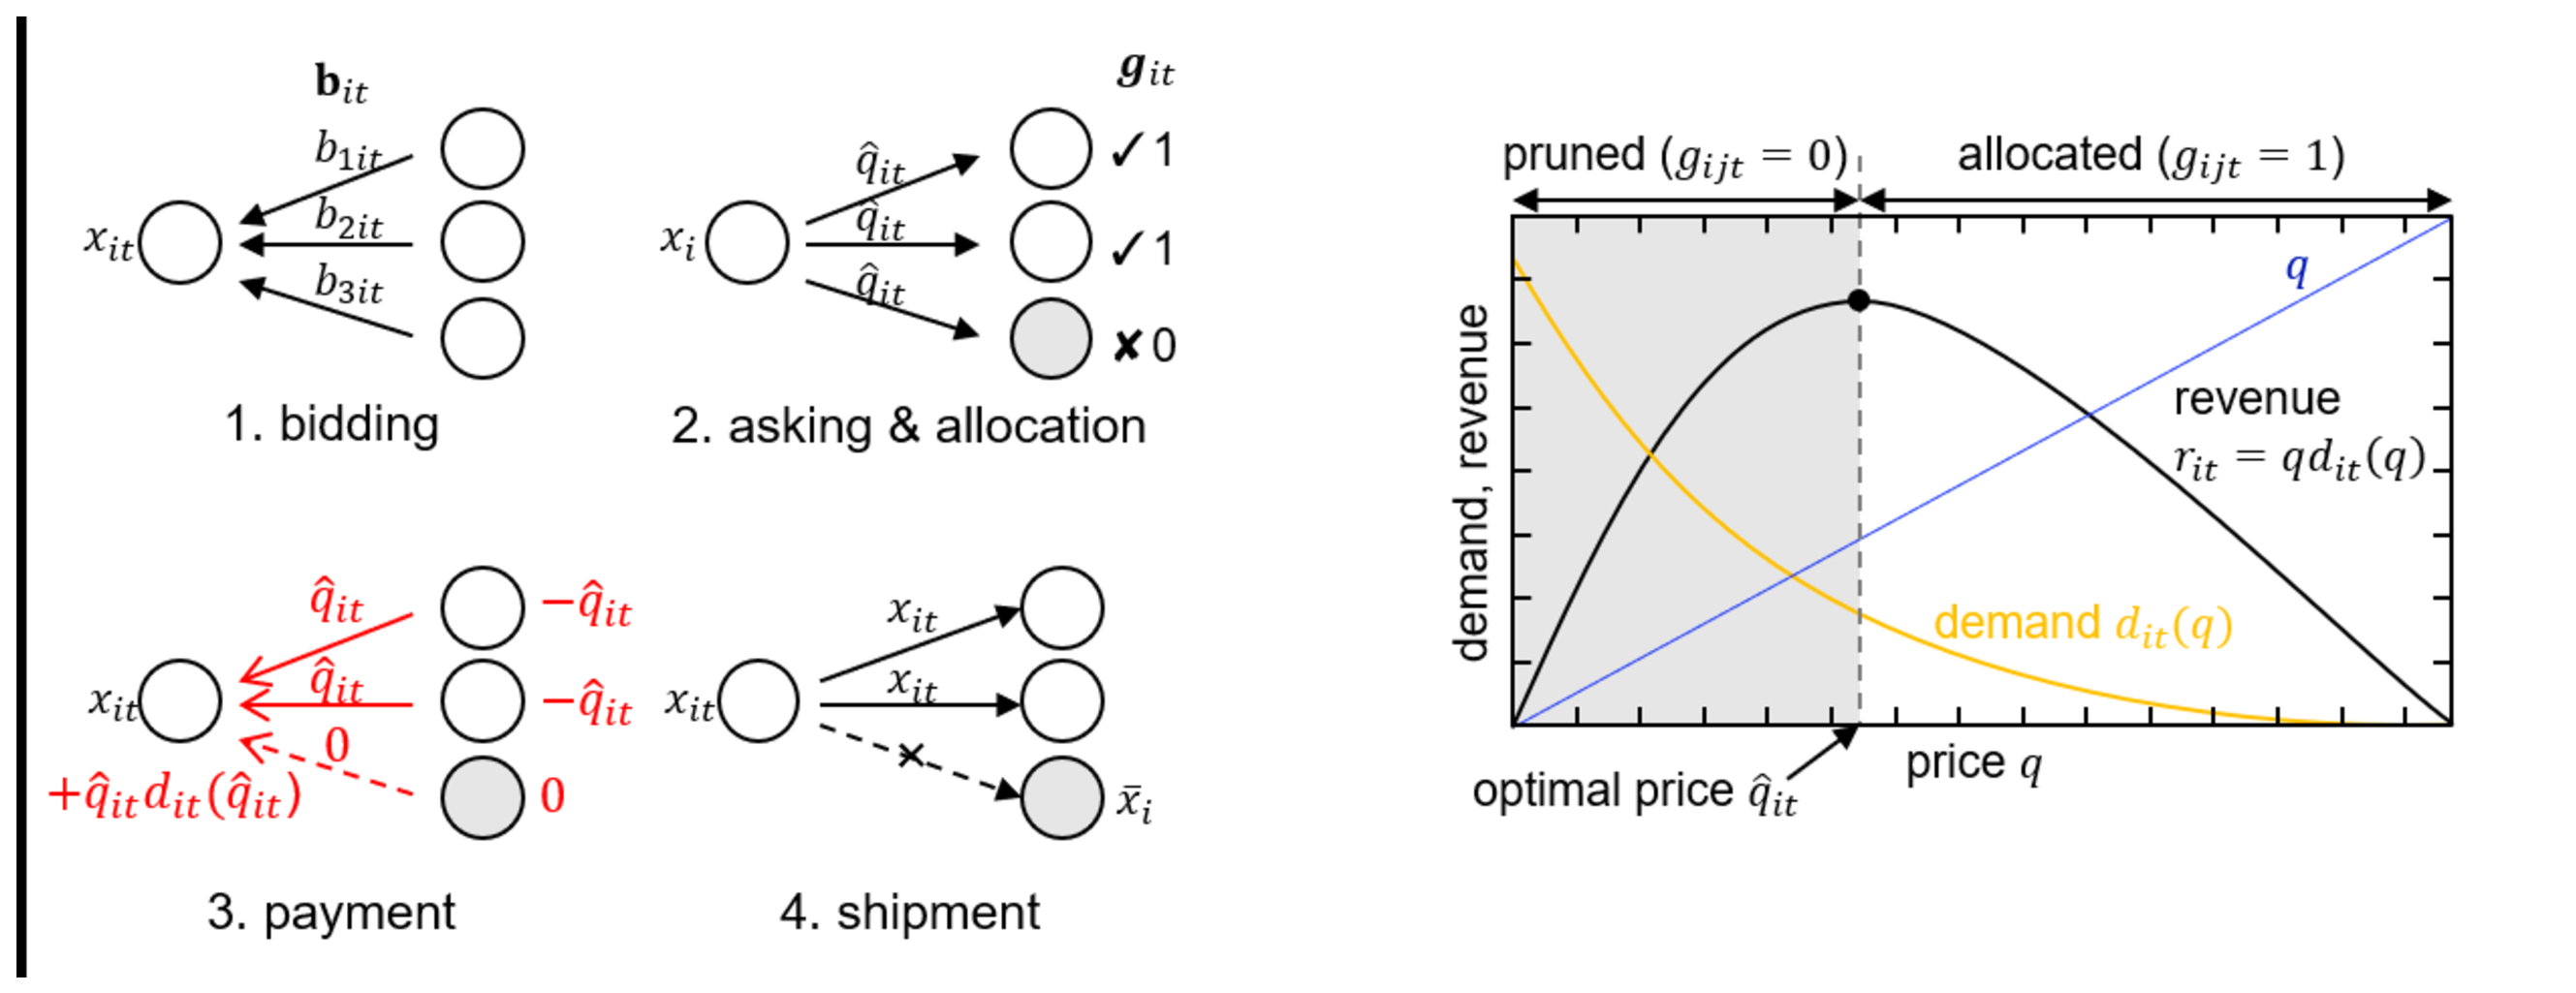
\includegraphics[width=\linewidth]{img/double.eps}
\caption{
\textbf{Left}: The process of trade in an envy-free auction.
\textbf{Right}: A price determination curve for a unit. Revenue of a unit is a product of monotonically decreasing demand and price. The price maximizing the revenue is the optimal price.
}
\label{fig:double}
\end{figure*}


Therefore, the optimization problem is presented below.
\begin{flalign}
	%\max_{\vect{b}, q} \Expect{\hat{\vect{q}}_t}{ V_i^{\pi_i}(s_{it}) } = 
		\max_{\vect{a} } Q_i(s_{it}, \vect{a} )  = 
		\max_q q d_{it}(q) - 
		\min_{\vect{b}} \Expect{\hat{\vect{q}}_t}{\vect{g}_{it}(\vect{b})^\T( \hat{\vect{q}}_t - \gamma \vect{o}_{it}  )} + \const,
		\label{Eq:optimization-probem}
\end{flalign}
where $\vect{a} = (\vect{b}, q)$.
Note that $\vect{g}_{it} = H(\vect{b} - \vect{q}_t)$.
We take the expectation $\Expect{\hat{\vect{q}}_t}{\cdot}$ 
because the asked price $\hat{\vect{q}}_t$ is unknown for $v_i$, except for $\hat{q}_{it}$, and $g_{iit} = 0$.

Then, what is bidding price $b_{it}$ to maximize return?
The following theorem holds.

\begin{thm}\label{thm:optimal-bidding}
	(Truthfulness) the optimal bidding price for maximizing return is $\opt{\vect{b}}_{it} = \gamma \vect{o}_{it}$.
\end{thm}
See the Appendix for the proof.

That is, the unit should only consider its counterfactual return (!).
If $\gamma = 0$, the case is equivalent to a case without auction. Hence, the bidding value raises if each unit consider long-time reward. 
Consequently, in the mechanism of NaaA, the unit obeys as if performing valuation to the other units, 
and declares the value truthfully.

Then, the following corollary holds:
\begin{coro}\label{coro:optimal-bidding}
	The Nash equilibrium of an envy-free auction $(\vect{b}_{it}, q_{it})$ is $(\vect{o}_{it}, \argmax_{q} q d_{it}(q))$.
\end{coro}

The remaining problem is how to predict $\vect{o}_t$.
Although several method can be applied to this problem,
we use $Q$-learning to predict $\vect{o}_t$.
As $\vect{o}_{it}$ is difference of two $Q$s, we approximate each of $Q$.
Other RL such as SARSA and A3C can be employed.
We parametrize the state with a vector $\vect{s}_t$ 
which contains input and weight.
$\epsilon$-greedy policy with $Q$-learning typically suppose that discrete actions
So, as an action, we employ allocation $g_{ijt}$ instead of $\vect{b}_{it}$ and $q_{it}$.
The overall algorithm is shown in Algorithm 1.

\begin{algorithm}[t]
\caption{NaaA: inter-agent reward distribution with envy-free auction}
\begin{algorithmic}[1]
	\FOR{ $t=1$ \TO $T$ }
		\STATE Compute a bidding price for every edge: \textbf{for} $(v_j, v_i) \in \edges$ \textbf{do}\
		$b_{ijt} \leftarrow Q^{\pi_i}( \vect{s}_{it}, \vect{e}_j) - Q^{\pi_i}( \vect{s}_{it}, \vect{0})$ 
		\STATE Compute an asking price for every node: \textbf{for} $\unit \in \units$ \textbf{do}\
		$\opt{q}_{it} \leftarrow \argmax_{q \in [0, \infty)} q d_{it}(q).$
		\FOR{$(v_i, v_j) \in \edges$}
				\STATE Compute allocation: $g_{jit} \leftarrow H(b_{jit} - \opt{q}_{it})$ 
				\STATE Compute the price the agent should pay: $\rho_{jit} \leftarrow g_{jit} \opt{q}_{it}$ 
		\ENDFOR
		\STATE Make a payment: \textbf{for} $\unit \in \units$ \textbf{do}\
		$R_{it} \leftarrow \sum_{j \in N^\mathrm{out}_i} \rho_{jit} 
				- \sum_{j \in N^\mathrm{in}_i} \rho_{ijt},$
		\STATE Make a shipment: \textbf{for} $\unit \in \units$ \textbf{do}\
		$\tilde{x}_{ijt} = g_{ijt} x_{ijt} + ( 1 - g_{ijt} ) \bar{x}_{ijt} $

		\FOR{$\unit \in \units$} 
			\STATE Observe external state $\vect{s}_{it}^{\mathrm ex}$
			\STATE $\vect{s}_{it} \leftarrow (\vect{s}_{it}^{\mathrm ex}, \vect{\tilde{x}}_{it}, \bs{\theta}_i)$,\
				where $\vect{\tilde{x}}_{it} = (\tilde{x}_{i1t}, \dots, \tilde{x}_{int})^\mathrm{T}$ and\
				$\bs{\theta}_i$ is $\unit$'s parameter.
			\STATE Sample action $a_{it}^{\mathrm ex} \sim \pi_i^{\mathrm ex}(\vect{s}_{it})$
			\STATE Receive external reward $R_{it} \leftarrow R_{it} + R_{it}^{\mathrm ex}(a_{it}^{\mathrm ex})$
			\STATE Update $Q^{\pi_i}$ under the manner of $Q$-learning by calculating the time difference (TD)-error 
		\ENDFOR
	\ENDFOR
\end{algorithmic}
\end{algorithm}


%========================================================================
% 【論旨】
% - Q-learning と \epsilon-greedy 方策による強化学習で最適化をする
%	 - 状態を入力と重みを用いてパラメトライズする
%	 - 行動として allocation \g を用いる
%	 - 報酬は profit: revenue と cost の差
%    - つまり、NaaA では結果的に全体としてパフォーマンスが向上するようコネクションを最適化する
% 	 - これはランダムにエッジを落とす dropconnect の拡張であり、より精度向上ができると考えられる。
% - NaaA に基づくネットワーク最適化を adaptive dropconnect と名付ける
%	 - 類似の事例として、過去に提案されている adaptive dropout はこれをより一般化した話
%	 - $\epsilon=0$ の場合には dropconnect と完全に等しくなる
% - Adaptive dropconnect は、強化学習以外にも応用可能
% 	 - 強化学習以外の場合は、報酬として正解に基づく 0/1 の情報を用いて、$gamma = 0$ とする。
% 	 - 実装上は層を入れ替えるだけなので簡単
% - アルゴリズム
%========================================================================

%$\vect{o}_t$ のみ用いた greedy な方策を用いると、
%方策として、$\epsilon$-greedy を用いた
%We use $\epslion-greedy$
%We show that pre $Q$ lead us t
%我々は $\epslion-greedy$ における探索は dropconnect であるため、
%adaptive dropconnect に等しいことを示す。
%
%$\epsilon$
%
%次に、adaptive dropconnect について述べる。
%
%Value of the value function $V(s_{i,t+1})$ depends on $s_{i,t+1}$.
%As we already defined, the internal environment of $v_i$ is a set of connected units,
%and the output of units affect to evaluation from the units, namely, weight of edges.
%As the learning rule of a typical artificial neural network obeys to law of Hebb, 
%the reward becomes lower because weight of unit which do not contribute
%the accuracy of output becomes lower.


\section{Experiment}
To confirm that NaaA works widely with machine learning tasks, we confirm our method of supervised
learning tasks as well as reinforcement learning tasks. As supervised learning tasks, we use
typical machine learning tasks such as image classification using MNIST, CIFAR-10, and SVHN.

As reinforcement tasks, we confirm single- and multi-agent environment. The single-agent environment
is from OpenAI Gym. We confirm the result using a simple reinforcement task: CartPole. In
multi-agent, we use ViZDoom, a 3D environment for reinforcement learning.

\subsection{Classification}
\subsubsection{Setup}
%This experiment verified the performance of two tasks: classification and single-agent reinforcement learning.
For classification, three types of datasets were used: MNIST, CIFAR-10, and STL-10. 
The given task was to predict the label of each image, and each dataset had a class number of 10.
The first dataset, MNIST, was a collection of black and white images of handwritten digits sized 28�~28. The training and test sets contained 60,000 and 10,000 example images, respectively. 
The CIFAR-10 dataset images were colored and sized 32�~32, and the assigned task was to predict what was shown in each picture. This dataset contained 6,000 images per class (5,000 for training and 1,000 for testing).
The STL-10 dataset was used for image recognition, and had 1,300 images for each class (500 training, 800 testing). Each image was sized 96�~96; however, for the experiment, the images were resized to 48�~48 because the greater resolution of this dataset (relative to the above datasets) required far more computing time and resources.

\subsubsection{Model}
Two models were compared in this experiment: DropConnect and Adaptive DropConnect (the model proposed in this paper). The baseline model was composed of two convolutional layers and two fully connected layers whose outputs are dropped out (we set the possibility as 0.5). The labels of input data were predicted using log-softmaxed values from the last fully connected layer. In the DropConnect and Adaptive DropConnect models, the first fully connected layer was replaced by a DropConnected and Adaptive DropConnected layer, respectively. It should be noted that the DropConnect model corresponded to the proposed method when $\varepsilon$ = 1.0, meaning agents did not perform their auctions but instead randomly masked their weights.

\subsubsection{Results}
The models were trained over ten epochs using the MNIST datasets, and were then evaluated using the test data. The CIFAR-10 and STL-10 epoch numbers were 20 and 40, respectively. Experiments were repeated 20 times for each condition, and the averages and standard deviations of error rates were  calculated. Results are shown in Table \ref{tbl:cls}. As expected, the Adaptive DropConnect model performed with a lower classification error rate than either the baseline or DropConnect models regardless of the given experimental datasets.


\begin{table}[h]
	\caption{ Experimental result for image classification tasks and single-agent RL }\label{tbl:cls}. 
\centering
\begin{tabular}{l|ccc|c}
\hline
		& MNIST & CIFAR-10 & STL-10 & CartPole \\
\hline
		DropConnect \citep{wan2013regularization}	&	1.72 $\pm$ 0.160	&	43.14 $\pm$ 1.335	&	50.92 $\pm$ 1.322 & 285 $\pm$ 21.5 \\
		Adaptive DropConnect	&	\textbf{1.36} $\pm$ 0.132	&	\textbf{39.84} $\pm$ 1.035	&	\textbf{42.17} $\pm$ 2.329 & \textbf{347} $\pm$ 29.4 \\
\hline
\end{tabular}
\end{table}

\subsection{Single-agent RL}
Next, the single-agent reinforcement learning task was set as 
the CartPole task from OpenAI Gym \citep{openaigym} with visual inputs.
In this setting, the agent was required to balance a pole while moving a cart.
The images contained a large amount of non-useful information, making pixel pruning important.
The result in Table \ref{tbl:cls} demonstrates that our method improves the standard RL.

\subsection{Multi-agent RL}
The proposed reward distribution method was confirmed to work as expected by a validation experiment using the multi-agent setting in ViZDoom \citep{kempka2016vizdoom}, 
an emulator of Doom containing a map editor where additional agents complement the main player.
A main player in the ViZDoom environment aims to seek the enemy in the map and then defeat the enemy.

\subsection{Setup}
A defend the center (DtC)-based scenario, provided by ViZDoom platform, was used for this experiment.
Two players, a main player and a cameraman, were placed in the DtC, where they started in the center of a circular field and then attacked enemies that came from the surrounding wall.
Although the main player could attack the enemy with bullets, 
the cameraman had no way to attack, only scouting for the enemy.
The action space for the main player was the combination of \{ attack, turn left, turn right \}, giving a total number of actions $2^3 = 8$.
The cameraman had two possible actions: \{ turn left, turn right \}.
Although the players could change direction, they could not move on the field.
Enemies died after receiving one attack (bullet) from the main player, and then player received a score of +1 for each successful attack.
The main player received 26 bullets by default at the beginning of each episode.
The main player died if they received attacks from the enemy to the extent that their health dropped to 0, and received a score of -1 for each death.
The cameraman did not die if attacked by an enemy.
Episodes terminated either when the maim player died or after 525 steps elapsed.

\subsection{Model}
Three models, described below, were compared: the proposed method and two comparison targets.

{\em Baseline}: DQN without communication. The main player learned standard DQN with the perspective that the player is viewing.
Because the cameraman did not learn, this player continued to move randomly.

{\em Comm}: DQN with communication, inspired by Commnet. The main player learns DQN with two perspectives: theirs and that of the cameraman.
The communication vector is learned with a feed-forward neural network.

{\em NaaA}: The proposed method. The main player learned DQN with two perspectives: theirs and that of the cameraman.
Transmissions of rewards and communications were performed using the proposed method.

\begin{figure*}[t]
\centering
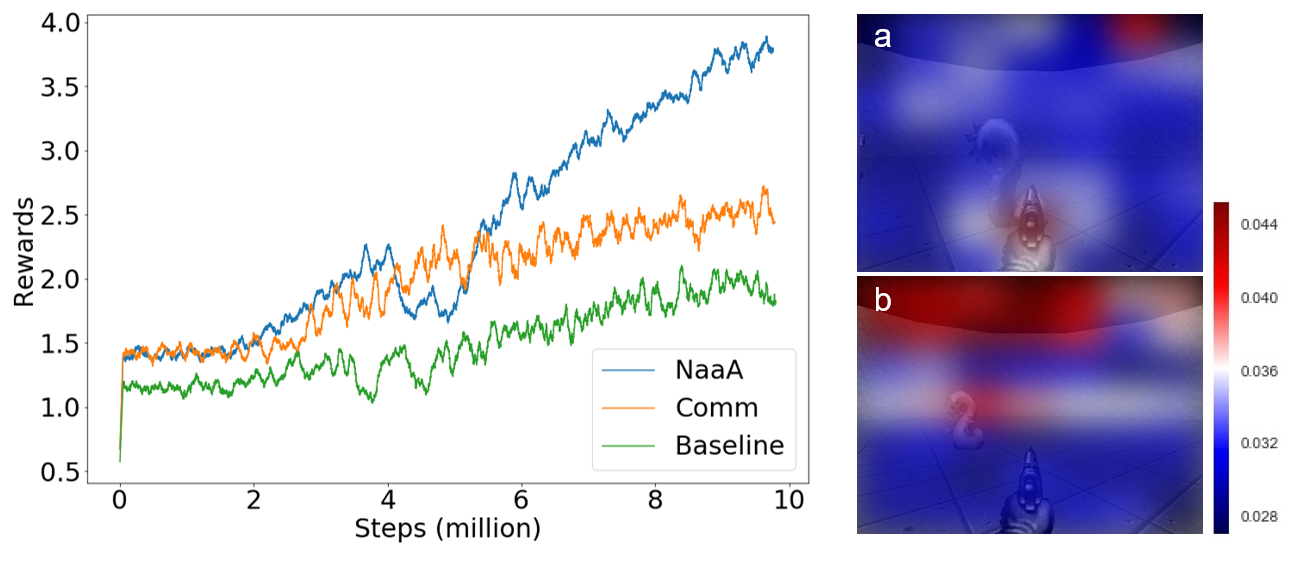
\includegraphics[width=\linewidth]{img/lc_vis.eps}
\caption{
	\textbf{Left:}
		Learning curve for ViZDoom multi-agent task. 
		The proposed NaaA--based method outperformed the other two methods (baseline and Comm DQNs).
	\textbf{Right:} 
		Visualizing reward from the main player to the cameramann shows us what is important information for the main player:
		(a) The pistol.
		(b) The point at which the enemy appeared and approached.
}
\label{fig:lc_vis}
\end{figure*}

\begin{figure*}[t]
\centering
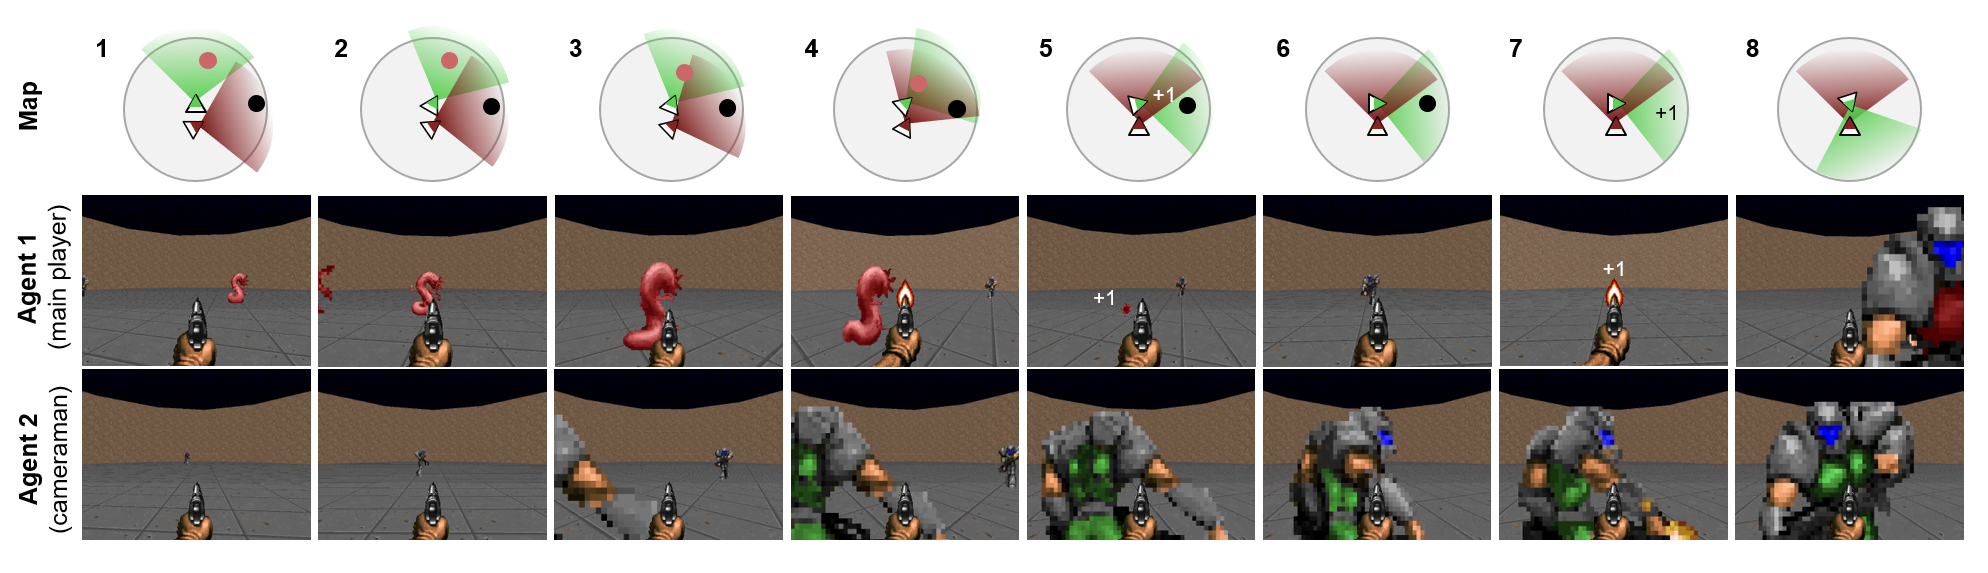
\includegraphics[width=\linewidth]{img/circleworld.eps}
\caption{
NaaA leads agents to enter a cooperative relationship.
First, the two agents face different directions,
and the cameraman sells their information to the main player (\textbf{1}).
The main player (information buyer) starts to turn right to find the enemy.
The cameraman (information seller) starts to turn left to seek new information by finding the blind area of the main player (\textbf{2} and \textbf{3}).
After turning, the main player attacks the first, having already identified enemy (\textbf{4} and \textbf{5}).
Once the main player finds the enemy, he attacks and obtains the reward (\textbf{6} and \textbf{7}).
Both agents then return to watching the dead area of the other until the next enemy appears (\textbf{8}).
}
\label{fig:circleworld}
\end{figure*}

\subsection{Results}
Training was performed over the course of 10 million steps.
Figure \ref{fig:lc_vis} Left demonstrates the proposed NaaA model outperformed the other two methods.
Improvement was achieved by Adaptive DropConnect.
It was confirmed that the cameraman observed the enemy through an episode, which could be interpreted as the cameraman reporting enemy positions.
In addition to seeing the enemy, the cameraman observed the area behind the main player several times.
This enabled the cameraman to observe enemy attacks while taking a better relative position.

To further interpret this result, 
a heatmap visualization of revenue earned by the agent is presented in Figure \ref{fig:lc_vis} Right.
The background picture is a screen from Doom, recorded at the moment when the CNN filter was most activated.
%The center corresponds to a position with the enemy appearing far away.
%The top corresponds to a position with the enemy coming closer.
%(b) shows that the agent sees the pistol.
Figure \ref{fig:circleworld} shows an example of learnt sequence of actions by our method.


%To confirm that NaaA works widely with machine learning tasks,
%we confirm our method of supervised learning tasks as well as reinforcement learning tasks.
%As supervised learning tasks, we use typical machine learning tasks such as image classification
%using MNIST, CIFAR-10, and SVHN.

%As reinforcement tasks, we confirm single- and multi-agent environment.
%The single-agent environment is from OpenAI gym.
%We confirm the result using a simple reinforcement task: CartPole.
%In multi-agent, we use ViZDoom, a 3D environment for reinforcement learning.

%The additional feature of NaaA is credit assignment for reward distribution, 
%meaning that if the neural network is divided into multiple agents, it works by playing the auction game.


\section{Related Work}
NaaA belongs to a class of partially observable stochastic game (POSG) \citep{hansen2004dynamic} because it processes multiple units as agents.
POSG, a class of reinforcement learning with multiple agents in a POMDP environment, presents several research issues, one of which is communication.
CommNet \citep{sukhbaatar2016learning}, which exploits the characteristics of a unit that is agnostic to the topology of other units, employs backpropagation to train multi-agent communication.
Another one is credit assignment.
Instead of reward $R(a_t)$ of an agent $i$ for actions at $t$ $a_t$, 
QUICR-learning \citep{agogino2006quicr} maximizes counterfactual reward $R(a_t) - R(a_t - a_{it})$, the difference in the case of the agent $i$ takes an action $a_{it}$ ($a_t$) and not ($a_t-a_{it}$).
COMA \citep{foerster2017counterfactual} also maximizes counterfactual rewards in an actor--critic setting.
In the setting, all actors have common critics, which improves both actors and critics with time difference (TD)-error of a counterfactual reward.
This paper unifies both issues: communication and credit assignment.
The main proposal is a framework to manage the agents to maximize the {\em counterfactual return}, the extended counterfactual reward along the time axis.

Training a neural network with a multi-agent game is an emerging methodology.
Generative adversarial nets (GAN) \citep{goodfellow2014generative} have the goal of obtaining true generative distribution as a Nash equilibrium of a competitive game that includes two agents with contradictory rewards: a generator and a discriminator. 
In game theory, the outcome maximizing overall reward is named Pareto optimality.
Nash equilibrium is not guaranteed to converge to Pareto optimality. The difference between them is designated as a dilemma.
Because the existence of a dilemma depends on the reward design, methods to resolve dilemmas with good reward design are being investigated: mechanism design \citep{myerson1983mechanism} is also known as inverse game theory.
Mechanism design is applied to auctions \citep{vickrey1961counterspeculation} and matching \citep{gale1962college}.
GAN and our proposal, NaaA, are outcomes from mechanism design.
NaaA applies a digital goods auction \citep{guruswami2005profit} to reinforcement learning with a multi-agent neural network, 
to obtain a maximized return by units as a Nash equilibrium.

Adaptive DropConnect (ADC) which we propose in a late part of this paper, extends DropConnect \citep{wan2013regularization}, a regularization technique.
The idea of ADC (instead of dropping each connection between the units in constant probability, using skew probability correlated to absolute value of weights) is eventually closer to Adaptive DropOut \citep{ba2013adaptive} although the derivation is different, 
and the adjective ``adaptive'' is added respecting the method.
Optimizing neural network with RL is investigated by \cite{andrychowicz2016learning}.
In contrast to their methods which uses recurrent neural network (RNN) and hence the implementation is difficult,
our method is RNN-free and forms as a layer, and hence the implementation is easy and fast, and it has wide applicable area.

\section{Discussion}
\subsection{Disadvantage}
\subsection{Shortcoming}
%An important shortcoming is its computational complexity.
%Because the envy-free auction uses a sort operation for computing demand,
%several parts should be serialized and should be improved through approximation.

Regarding the optimization method,
although envy-free auction guarantees truthfulness if the buyer prices are sealed,
in cases where buyers can mutually communicate and share price information, 
the buyer can fake the price with lower demand in a process of collusion.
To address the issue, several solutions such as random sample auction \cite{goldberg2006competitive} are proposed.

%Adaptive dropconnect has difficulty for implementation for several neural networks.
%Although we published source code on GitHub for Linear, 
%implementation for RNN remains as a subject for future work.

% Dropconnect: Theoertical background 

\subsection{Application}
NaaA is applicable to learning distributed environments on a computer network such as a peer-to-peer network, and controlling the sub-modules of robots such as multiple cameras.
Specifically, it is applicable to various methods as described below.
\begin{itemize}
\item Hyperparameter tuning. 
Several algorithms have been proposed such as neuroevolution using genetic algorithms.
In the case, profit or counterfactual return is useful for a fitness function.
\item Pruning. Computing costs can be reduced by downsizing a neural network.
\item Attention control. Research of attention is using reinforcement learning to control attention.
\item Ensemble. Our method is applicable to mixed multiple models.

% On-policy DropConnect
% Theoretical Analysis for Adaptive DropConnect
% Attention and sensor placement 
% Graph-based Algorithm such as PageRank
% Application to genrrative model
% Biological interpretation
\end{itemize}
These applications illustrate the direction of our research.

%\section{Conclusion and Future Works}
\section{Concluding Remarks and Future Work}
This paper proposed a NaaA model to address communication in MARL without a TTP based on two key ideas: inter-agent reward distribution and auction theory.
Existing MARL communication methods have assumed the existence of a TTP, and hence could not be applied in peer--to--peer environments.
The inter-agent reward distribution, making agents redistribute the rewards they received from the internal/external environment, was reviewed first.
When an envy-free auction was introduced using auction theory, it was shown that agents would evaluate the counterfactual returns of other agents.
The experimental results demonstrated that NaaA outperformed a baseline method and a CommNet-based method.

Furthermore, a $Q$-learning based algorithm, termed Adaptive DropConnect, was proposed to dynamically optimize neural network topology with counterfactual return evaluation as a further application.
To evaluate this application, experiments were performed based on a single-agent platform, demonstrating that the proposed method produced improved experimental results relative to existing methods.

% TODO: ���������ꍇ�̑΍�͂ǂ����ɏ���������������������Ȃ�

Future research may also be directed toward considering the connection between NaaA and neuroscience or neuroevolution.
Edeleman propounded the concept of neural Darwinism \citep{edelman1987neural}, in which group selection occurs in the brain.
Inter-agent rewards, which were assumed in this paper, correspond to NTFs
and could be used as a fitness function in genetic algorithms for neuroevolution such as hyperparameter tuning.

As NaaA can be applied in peer-to-peer environments, 
the implementation of NaaA in blockchain \citep{swan2015blockchain} is under consideration.
This implementation would extend the areas where deep reinforcement learning could be applied.
Bitcoin \citep{nakamoto2008bitcoin} could be used for inter-agent reward distribution, and the auction mechanism could be implemented by smart contracts \citep{buterin2014next}.
Using the NaaA reward design, it is hoped that the world may be united, allowing people to share their own representations on a global scale.

%We can use bitcoin \cite{nakamoto2008bitcoin} and smart contract \cite{}a 

%Besides, we proposed Adaptive DropConnect as an further application on a single neural network.
%This paper proposed NaaA, a reinforcement learning framework that treats each unit on a neural network as an agent.
%First, we pointed out there are dilemma problems if we naively optimize NaaA. 
%We proposed an optimization method with auction.
%Consequently, an action by which units evaluate the counterfactual return of other units is obtained as a Nash equilibrium.
%Furthermore, we proposed $Q$-learning based algorithm, adaptive dropconnect, to optimize the neural network topology dynamically with evaluation of counterfactual return.
%For the evaluation, we performed experiments based on single-agent and multi-agent platforms, demonstrating that our experimentally obtained results improve existing methods.

%As a direction of future research, we use on-policy methods to perform adaptive dropconnect, and
%consider applications combining genetic algorithms.


\bibliography{daisy}
\bibliographystyle{iclr2018_conference}

\appendix
\section*{Appendix}

% Set numbering of section alphabet: A, B, C,...
\setcounter{section}{1}
\renewcommand{\thesection}{\Alph{section}}

% Contents is started from here
%\subsection{Proof}
%We first proof $\rho_{ijt} = 0$ is the Nash equilibrium.
%The value function can be written as $r_{it} - c_{it} + \gamma V_{i,t+1}$.
%At the point, as other agents plays $\rho_{ijt} = 0$, the value function is $- c_{it}$.
%To maximizing this equation, $\rho_{ijt} = 0$ holds. 

\subsection{Proof of Theorem \ref{thm:optimal-bidding}}
As for a buyer, the asking price $\ask$ for a seller is unknown,
we address $\ask$ which has support $[0, \infty)$,
and consideration to maximize $\Expect{q}{G(b,q)}$,
In this case, the following equation holds.
\begin{flalign}
\deriv{b}{}\Expect{q}{G(b,q)} 
&= \deriv{b}{}\int_0^\infty (H(b - q) \cdot (v-q) + G_0) p(q) dq \notag \\
&= \deriv{b}{} \left[ \int_0^b (v-q) p(q) dq + G_0 \int_0^\infty p(q)dq \right] \notag \\
&= \deriv{b}{} \int_0^b (v-q) p(q) dq \notag \\
&= (v-b) p(q=b), \notag 
\end{flalign}
Therefore, the condition to maximize $\Expect{q}{G(b,q)}$ is $b=v$.


\end{document}

